\documentclass[11pt]{article}

\usepackage[margin=1in]{geometry}
\usepackage{array}
\usepackage{booktabs}
\usepackage{float}
\usepackage{graphicx}
\usepackage{hyperref}
\hypersetup{hidelinks}
\graphicspath{{report/}{./}}

\title{Edge-Cloud Vision System for Meta Quest 3S Using a Wi-Fi-Connected GPU Backend}
\author{Hoang Phuc Nguyen \\ Hung Luong Duc}
\date{CSE 422 Honors Option}

\begin{document}

\maketitle

\begin{abstract}
This project implements an end-to-end edge-cloud vision system for a Meta Quest 3S mixed-reality headset. The headset captures camera frames in Unity, compresses each frame as a JPEG image, and sends it over a Wi-Fi TCP connection to a local GPU backend. The Python backend decodes the image, runs YOLO segmentation on an NVIDIA GPU, and returns labels, bounding boxes, and optional mask polygons as newline-delimited JSON. Unity parses the response and renders labeled 2D bounding boxes over the camera preview. The system was demonstrated successfully in a recorded mixed-reality demo. A 100-frame localhost protocol sanity test, not a headset Wi-Fi latency result, achieved a median round-trip time of 27.98 ms with a persistent TCP connection. The live demo showed the main practical limitation: bounding boxes update with a small visible delay.
\end{abstract}

\section{System Overview}

The goal of the project was to build a working distributed vision pipeline that connects a resource-constrained XR client to a more powerful GPU backend. The final system uses the Meta Quest 3S as the client and a local laptop with an NVIDIA RTX 4070 Laptop GPU as the inference server.

The end-to-end pipeline is:

\begin{enumerate}
    \item Unity on the Quest captures a passthrough camera frame.
    \item The client downsizes the image to the target resolution and encodes it as JPEG.
    \item The client sends a 4-byte little-endian payload length followed by the JPEG bytes over TCP.
    \item The Python backend decodes the image and runs YOLO segmentation on the GPU.
    \item The server sends one newline-terminated JSON response containing detections.
    \item Unity parses the JSON and draws labeled bounding boxes over the preview image.
\end{enumerate}

\begin{table}[h]
\centering
\begin{tabular}{>{\raggedright\arraybackslash}p{0.24\linewidth} >{\raggedright\arraybackslash}p{0.28\linewidth} >{\raggedright\arraybackslash}p{0.34\linewidth}}
\toprule
\textbf{Stage} & \textbf{Component} & \textbf{Network/Data Role} \\
\midrule
Capture & Quest 3S Unity client & Produces camera frame for transmission. \\
Compression & Unity client & Encodes frame as JPEG to reduce payload size. \\
Request transport & TCP socket & Sends length-prefixed image payload reliably and in order. \\
Inference & Python GPU backend & Decodes request, runs model, builds detection response. \\
Response transport & TCP socket & Sends one JSON line per processed frame. \\
Visualization & Unity client & Draws labels and bounding boxes from server response. \\
\bottomrule
\end{tabular}
\caption{End-to-end architecture and data flow.}
\end{table}

\subsection{Network Topology}

The final demo used an approved local GPU machine instead of the originally described campus GPU server. This changed the networking environment from remote campus/server routing to a local LAN Wi-Fi setup.

\begin{itemize}
    \item \textbf{Client:} Meta Quest 3S headset \cite{meta-quest3s}.
    \item \textbf{Backend:} Lenovo laptop on the same Wi-Fi LAN.
    \item \textbf{Backend bind address:} \texttt{0.0.0.0:40081}, so the service accepts remote LAN connections.
    \item \textbf{Observed LAN addressing during debugging:} Quest at \texttt{192.168.50.75/24}, backend at \texttt{192.168.50.143/24}.
    \item \textbf{Observed Wi-Fi link:} same SSID and 5 GHz channel, with Wi-Fi 6 reported by the headset diagnostics. Wi-Fi 6 is the 802.11ax generation of Wi-Fi \cite{wifi6}.
    \item \textbf{NAT traversal:} not required, because the client and backend were on the same private subnet.
\end{itemize}

\begin{figure}[h]
\centering
\fbox{%
\begin{minipage}{0.88\linewidth}
\centering
\texttt{Meta Quest 3S Unity client}\\
\texttt{capture + JPEG encode}\\[0.5em]
\(\Downarrow\) \texttt{Wi-Fi TCP request: [4-byte length][JPEG bytes]}\\[0.5em]
\texttt{Local laptop backend, 0.0.0.0:40081}\\
\texttt{asyncio receive + GPU segmentation}\\[0.5em]
\(\Uparrow\) \texttt{Wi-Fi TCP response: one JSON line}\\[0.5em]
\texttt{Unity JSON parse + pooled bounding-box overlay}
\end{minipage}}
\caption{Network path and request/response flow for one processed frame.}
\end{figure}

\section{Network Design}

The network layer uses a custom TCP request/response protocol. TCP was chosen for this minimum viable prototype (MVP) because it gives \cite{rfc9293}:

\begin{itemize}
    \item reliable delivery of each complete image frame;
    \item ordered delivery, so responses stay associated with the frame order;
    \item simpler debugging than an unreliable transport;
    \item a natural request/response model: send one frame, receive one result.
\end{itemize}

The protocol uses explicit application-level framing:

\begin{itemize}
    \item \textbf{Request header:} 4-byte little-endian integer containing the JPEG payload length.
    \item \textbf{Request body:} exactly that many JPEG bytes.
    \item \textbf{Response:} one UTF-8 JSON object terminated by a newline.
\end{itemize}

This framing is necessary because TCP is a byte stream, not a message protocol. The length prefix tells the server exactly how many bytes belong to the current image. The newline delimiter lets Unity find the end of the JSON response without needing a second response-length header.

The wire format is:

\begin{verbatim}
Client -> Server:
[4-byte little-endian length N][N JPEG bytes]

Server -> Client:
{"frame_id":17,"status":"ok","latency_ms":31.2,"detections":[...]}
\n
\end{verbatim}

Important protocol and socket parameters are:

\begin{table}[h]
\centering
\begin{tabular}{>{\raggedright\arraybackslash}p{0.31\linewidth} >{\raggedright\arraybackslash}p{0.56\linewidth}}
\toprule
\textbf{Parameter} & \textbf{Value / Purpose} \\
\midrule
Backend port & \texttt{40081}. \\
Server bind address & \texttt{0.0.0.0}, allowing LAN clients to connect. \\
Maximum frame size & 10 MiB on the backend to reject malformed or oversized requests. \\
Client response cap & 262,144 bytes to avoid unbounded JSON reads. \\
Client socket timeout & 10,000 ms for connect/read/write operations. \\
TCP no-delay & Enabled on the Unity client; Python asyncio also enables \texttt{TCP\_NODELAY} by default for TCP connections in modern Python \cite{python-asyncio-eventloop}. \\
Capture payload & 640\(\times\)480 JPEG, quality 60 in the Unity client. \\
Send interval & 0.5 s by default, so the live client attempts about 2 processed frames per second. \\
Server sequence ID & Each response includes a server-generated \texttt{frame\_id} and status field. The current request format does not include a client-generated frame ID or timestamp. \\
\bottomrule
\end{tabular}
\caption{Protocol and socket parameters used by the client/server system.}
\end{table}

The 10,000 ms socket timeout is a safety timeout for detecting stalled connections. It is not the target latency for mixed reality. A production version should discard or fade responses that exceed a much smaller freshness threshold.

The client keeps one frame in flight at a time. This is an intentional flow-control decision:

\begin{itemize}
    \item If Unity sent frames faster than the backend could process them, stale frames would queue up.
    \item Stale detections could then be drawn over the current live camera view.
    \item One frame in flight lowers throughput, but it keeps latency and visual correctness easier to reason about.
\end{itemize}

The Unity client also keeps a persistent TCP connection during a sending session:

\begin{itemize}
    \item Reusing one connection avoids repeating TCP setup for every frame.
    \item The server can maintain naturally increasing frame identifiers across a run.
    \item If the socket fails, the client closes it and reconnects on the next send attempt.
\end{itemize}

One practical network issue occurred during integration:

\begin{itemize}
    \item Windows marked the Wi-Fi network as a public network.
    \item The public firewall profile blocked inbound headset connections even though the backend was listening on port 40081.
    \item The server was reachable locally, but remote clients on the same subnet timed out.
    \item Setting the Wi-Fi network profile to Private and/or adding an inbound firewall rule for TCP port 40081 resolved the timeout.
\end{itemize}

The main tradeoff is reliability versus freshness:

\begin{itemize}
    \item TCP gives reliable delivery and simple frame boundaries.
    \item Mixed-reality visuals are time-sensitive.
    \item If capture, encoding, network transfer, or inference takes too long, the bounding box can be correct for an older frame but appear delayed relative to the live view.
\end{itemize}

TCP head-of-line blocking is an important limitation. If a segment of a JPEG frame is lost, later bytes cannot be delivered to the application until the missing data is retransmitted. This is acceptable for the MVP because the client sends only one frame at a time, so there is no large queue of later frames waiting behind a lost packet. If the system allowed multiple frames in flight, TCP head-of-line blocking could make stale detections accumulate.

\begin{table}[H]
\centering
\begin{tabular}{>{\raggedright\arraybackslash}p{0.18\linewidth} >{\raggedright\arraybackslash}p{0.35\linewidth} >{\raggedright\arraybackslash}p{0.35\linewidth}}
\toprule
\textbf{Transport} & \textbf{Advantage} & \textbf{Drawback} \\
\midrule
TCP & Reliable, ordered, simple to debug, easy request/response framing. & Head-of-line blocking; late frames are still delivered. \\
UDP & Can drop stale frames and avoid retransmission delay. & Requires custom reliability, ordering, and loss handling if needed. \\
WebSocket & Convenient message abstraction over TCP. & Still inherits TCP head-of-line blocking. \\
WebRTC/video & Designed for real-time media and congestion control \cite{webrtc-overview}. & More complex and harder to attach simple per-frame inference metadata. \\
\bottomrule
\end{tabular}
\caption{Transport tradeoffs for the MR vision pipeline.}
\end{table}

\section{Backend and Client Implementation}

The backend implementation is responsible for receiving frames and running inference:

\begin{itemize}
    \item Python asyncio TCP server.
    \item Reads length-prefixed image frames from each client.
    \item Decodes JPEG images with Pillow.
    \item Runs YOLO segmentation through Ultralytics \cite{ultralytics-yolo26}.
    \item Loads the model once at server startup, not once per frame.
    \item Uses \texttt{--no-frame-log} during live runs to avoid disk I/O latency.
\end{itemize}

Each detection response includes:

\begin{itemize}
    \item frame identifier and status;
    \item received byte count and decoded image size;
    \item model name and backend inference latency;
    \item detection class labels and confidence scores;
    \item bounding boxes in decoded image coordinates as \texttt{[x\_min, y\_min, x\_max, y\_max]};
    \item optional segmentation mask polygons.
\end{itemize}

For the live headset overlay, Unity uses the labels and bounding boxes. Mask polygons are kept in the server response for debugging and offline annotated outputs, but live mask rendering is optional and not required for the demonstrated result.

The Unity client is responsible for capture, networking, and visualization:

\begin{itemize}
    \item Runs on the Meta Quest 3S.
    \item Uses asynchronous GPU readback instead of the older blocking readback path \cite{unity-asyncgpu}.
    \item Encodes JPEG data on a background task.
    \item Uses a persistent \texttt{TcpClient}.
    \item Parses JSON responses with Newtonsoft JSON.
    \item Draws pooled UI bounding boxes and labels over the preview image.
\end{itemize}

\subsection{Overlay Coordinate Mapping}

The server returns bounding boxes in decoded image pixel coordinates:

\begin{itemize}
    \item origin at the top-left of the decoded image;
    \item \(x\) increasing to the right;
    \item \(y\) increasing downward;
    \item coordinates measured against the server-reported image width and height.
\end{itemize}

Unity maps those boxes onto the preview UI as follows:

\begin{itemize}
    \item Normalize each coordinate by the decoded image width and height.
    \item Compute the displayed image rectangle inside the \texttt{RawImage} using the image aspect ratio and the UI container aspect ratio.
    \item Apply letterbox or pillarbox offsets before placing the overlay.
    \item Convert from image top-left coordinates to Unity UI coordinates by flipping the vertical axis.
    \item Apply optional mirror-X, mirror-Y, and rotation calibration values for headset/camera orientation differences.
    \item Place the label at the top-left of the box, moving it inside the box if the label would go above the preview.
\end{itemize}

The demo calibration values were:

\begin{itemize}
    \item mirror-X disabled;
    \item mirror-Y disabled;
    \item overlay rotation set to none;
    \item mask polygon drawing disabled for the live demo.
\end{itemize}

\subsection{Test Coverage}

The backend repository includes automated tests for the main protocol and server behavior:

\begin{itemize}
    \item frame-length packing and unpacking;
    \item JSON serialization for detections, empty detections, and error responses;
    \item fake-detector tests that avoid requiring a GPU during unit tests;
    \item async server integration tests that send an encoded image and verify the JSON response;
    \item evaluation-script helper tests for CSV/JSON output and TCP response parsing.
\end{itemize}

\section{Evaluation}

\subsection{Hardware and Demo}

The evaluation used the following hardware:

\begin{itemize}
    \item \textbf{Headset:} Meta Quest 3S.
    \item \textbf{Backend machine:} Lenovo laptop.
    \item \textbf{CPU:} AMD Ryzen 7 8845HS.
    \item \textbf{Memory:} 32 GB RAM.
    \item \textbf{GPU:} NVIDIA GeForce RTX 4070 Laptop GPU.
    \item \textbf{Inference device:} CUDA was available during evaluation \cite{nvidia-cuda}.
\end{itemize}

The instructor allowed the use of the local computer for the final implementation.

The recorded demo confirmed the end-to-end system:

\begin{itemize}
    \item The submitted demo video is about 94.1 seconds long at 2560\(\times\)1368 resolution.
    \item Demo video submitted with the report: \texttt{Casting \_ Meta Horizon - Google Chrome 2026-05-05 20-18-44.mp4}.
    \item Unity sent frames from the Quest to the backend.
    \item The backend returned detection results.
    \item Unity rendered labeled bounding boxes in mixed reality.
    \item No crashes, socket failures, or visible parsing/rendering failures were observed in the recorded demo.
    \item The visible limitation was that bounding boxes took a small amount of time to update.
\end{itemize}

\begin{figure}[H]
\centering
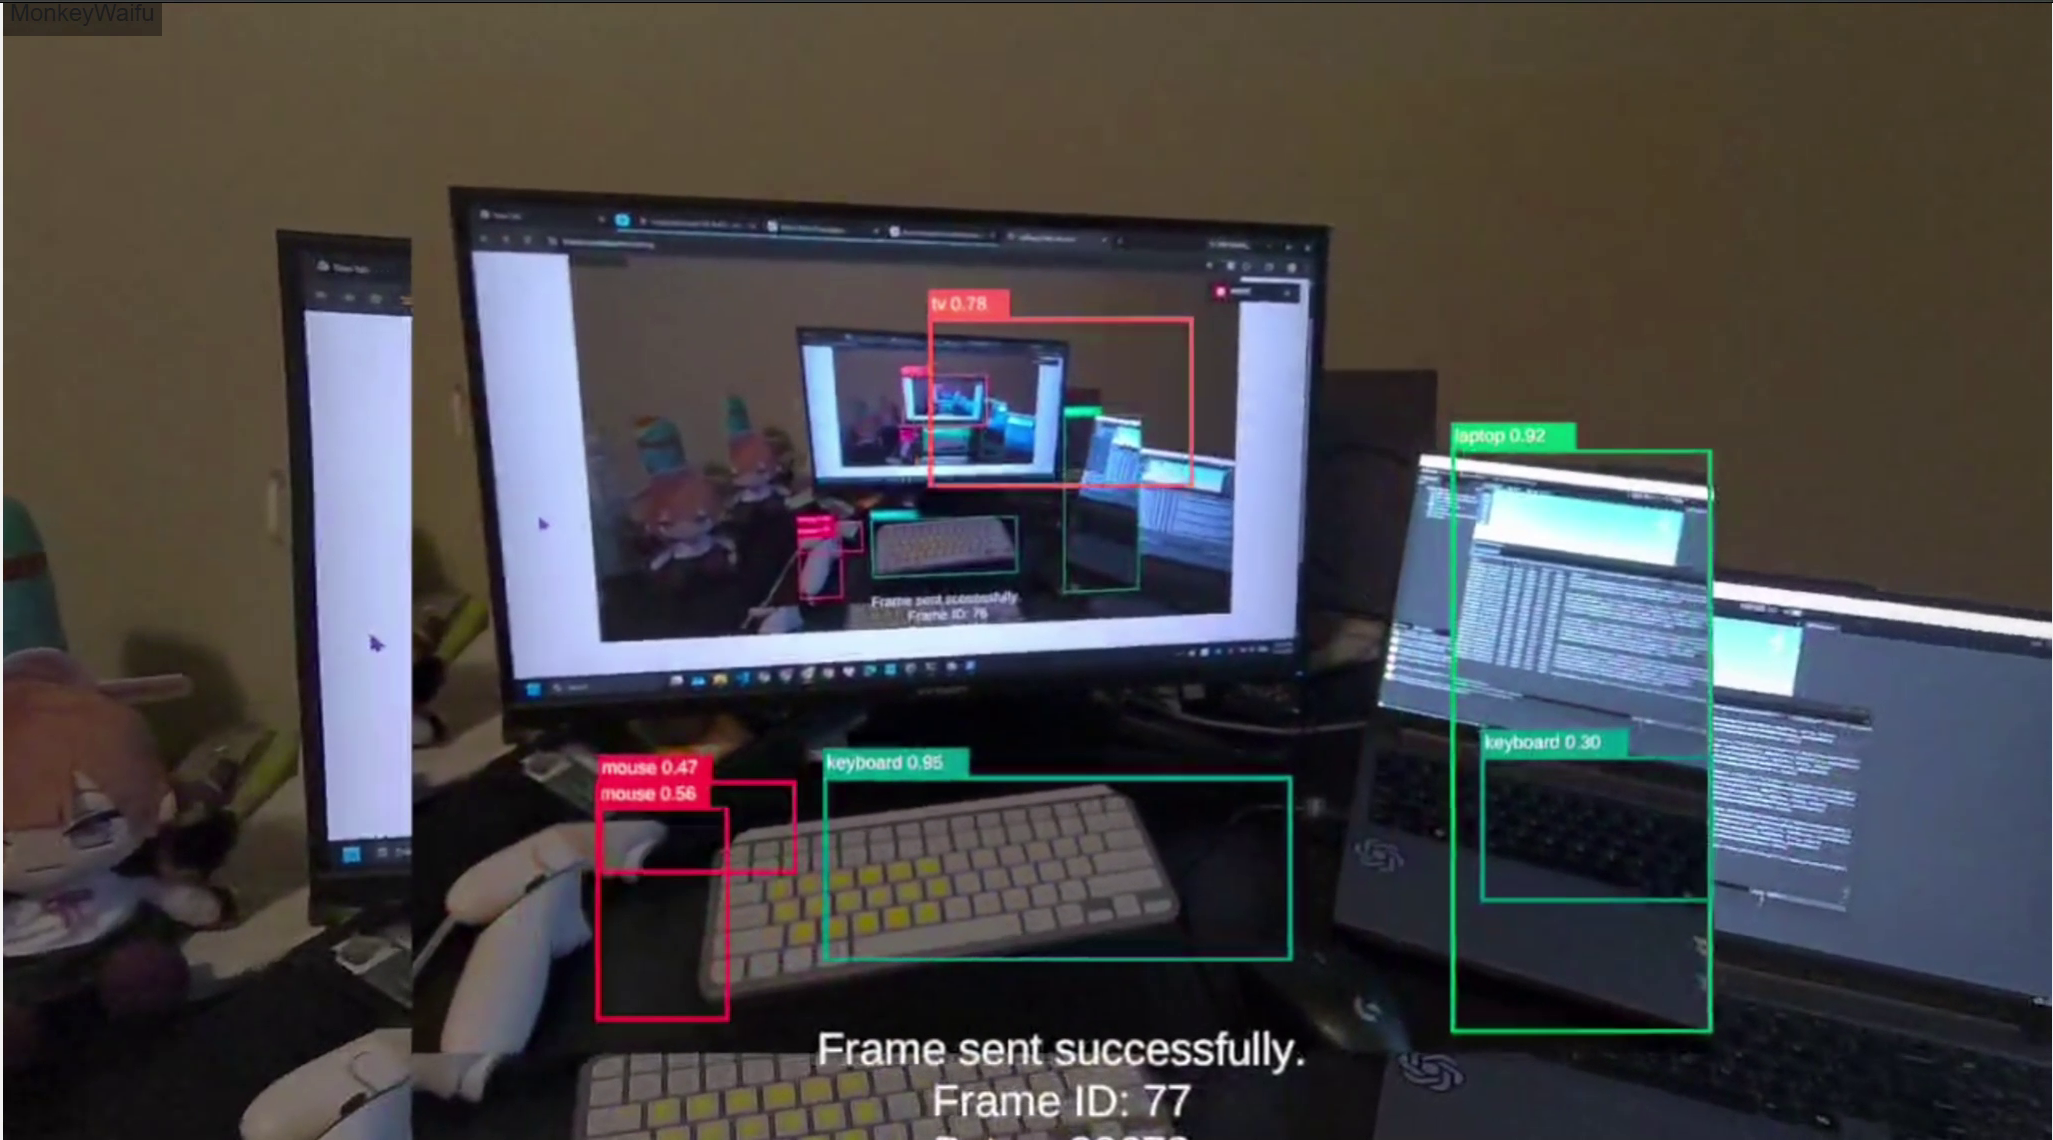
\includegraphics[width=0.86\linewidth]{demo_bounding_boxes_cropped.png}
\caption{Frame extracted from the recorded demo showing the live Unity overlay with labels and bounding boxes.}
\end{figure}

One captured frame from the demo showed a readback time of about 41.8 ms. This should be interpreted as GPU readback wall time, not necessarily a full main-thread stall, because the implementation yields while waiting for asynchronous GPU readback.

The backend and evaluation test suite passed:

\begin{center}
\texttt{Ran 18 tests \quad OK}
\end{center}

\subsection{Measurement Scope}

The evaluation separates three different types of evidence:

\begin{table}[h]
\centering
\begin{tabular}{>{\raggedright\arraybackslash}p{0.24\linewidth} >{\raggedright\arraybackslash}p{0.32\linewidth} >{\raggedright\arraybackslash}p{0.30\linewidth}}
\toprule
\textbf{Measurement} & \textbf{What it Shows} & \textbf{Limitation} \\
\midrule
Recorded Quest demo & Confirms real Wi-Fi end-to-end functionality and visible overlay rendering. & Does not provide per-frame RTT, jitter, or retransmission logs. \\
Saved-frame inference & Measures GPU/backend inference and response size without network variability. & Does not include headset capture or Wi-Fi transfer. \\
Local TCP sanity test & Measures protocol overhead, request/response stability, and persistent-vs-reconnect behavior. & Runs on \texttt{127.0.0.1}, so it is not a Wi-Fi performance test. \\
\bottomrule
\end{tabular}
\caption{Scope of the collected measurements.}
\end{table}

The main missing network measurement is a live per-frame Wi-Fi log from the Quest. The demo proved the Wi-Fi path worked, but it did not record enough samples to compute live wireless RTT, jitter, packet retransmissions, or reconnect rate. For that reason, the report does not claim that the localhost TCP numbers represent headset Wi-Fi performance. This remains the largest evaluation weakness.

A small future headset-side log would close the biggest evaluation gap:

\begin{itemize}
    \item server sequence ID from the response;
    \item Unity timestamp immediately before socket write;
    \item Unity timestamp immediately after the JSON line is received;
    \item server-reported processing latency from the JSON response;
    \item client-observed RTT and reconnect/failure status for each frame.
\end{itemize}

\subsection{Saved-Frame Inference}

Saved camera frames from the Quest were used to measure backend inference latency and response size without live headset or Wi-Fi variability. The first frame includes model/CUDA warm-up, so median latency and warm-up-excluded mean latency are more representative than the raw mean.

The saved JPEG request sizes were:

\begin{itemize}
    \item mean JPEG size: 43,719 bytes;
    \item median JPEG size: 38,283 bytes;
    \item minimum JPEG size: 22,794 bytes;
    \item maximum JPEG size: 59,910 bytes.
\end{itemize}

\begin{table}[H]
\centering
\small
\begin{tabular}{@{}lrrrrr@{}}
\toprule
\textbf{Model} & \textbf{Frames} & \textbf{Median} & \textbf{Mean*} & \textbf{Avg. Resp.} & \textbf{Avg. Det.} \\
 & & \textbf{(ms)} & \textbf{(ms)} & \textbf{(bytes)} & \\
\midrule
\texttt{yolo26s-seg.pt} & 19 & 30.75 & 32.45 & 5,690.84 & 2.105 \\
\texttt{yolo26n-seg.pt} & 19 & 36.80 & 37.09 & 4,676.00 & 2.368 \\
\bottomrule
\end{tabular}
\caption{Saved-frame backend inference results. The mean latency column excludes the first warm-up frame.}
\end{table}

The filenames \texttt{yolo26s-seg.pt} and \texttt{yolo26n-seg.pt} are the Ultralytics YOLO26 segmentation checkpoints used in this project, not custom names or report shorthand \cite{ultralytics-yolo26}. In this dataset, \texttt{yolo26s-seg.pt} had the better steady-state latency, while \texttt{yolo26n-seg.pt} produced slightly smaller responses on average. Because this was only a 19-frame saved-frame run with GPU warm-up and scheduling effects, this result should not be interpreted as a general model-speed ranking. Response size varied depending on the number of detections and the size of segmentation mask polygons.

\subsection{Bandwidth Demand Estimate}

The Unity client uses a default send interval of 0.5 s, or about 2 processed frames per second when the backend keeps up. Using the measured persistent TCP request/response sizes, the approximate application-level bandwidth demand is:

Uplink Mbps = frames/s \(\times\) request bytes \(\times 8 / 1{,}000{,}000\). Downlink Mbps = frames/s \(\times\) response bytes \(\times 8 / 1{,}000{,}000\). The response sizes used here are from the current segmentation JSON response, which can include mask polygons; a boxes-only live response would reduce downlink bandwidth.

\begin{table}[H]
\centering
\begin{tabular}{rrrr}
\toprule
\textbf{Processed Frame Rate} & \textbf{Uplink} & \textbf{Downlink} & \textbf{Total} \\
\textbf{(frames/s)} & \textbf{(Mbps)} & \textbf{(Mbps)} & \textbf{(Mbps)} \\
\midrule
2 & 0.695 & 0.088 & 0.783 \\
5 & 1.737 & 0.220 & 1.956 \\
10 & 3.473 & 0.440 & 3.913 \\
\bottomrule
\end{tabular}
\caption{Estimated application-level bandwidth demand from measured request and response sizes.}
\end{table}

These numbers are small compared with typical Wi-Fi 6 link capacity. This suggests that bandwidth was unlikely to be the primary bottleneck at the current frame rate. The more important network concerns are delay, jitter, retransmission behavior, and whether late results become visually stale.

\subsection{Local TCP Protocol Sanity Test}

A local TCP test sent saved frames to the running backend using the same protocol as Unity:

\begin{itemize}
    \item 4-byte little-endian frame length;
    \item JPEG payload bytes;
    \item newline-terminated JSON response.
\end{itemize}

This test was run on \texttt{127.0.0.1}. It measures backend protocol overhead and server stability, not real headset Wi-Fi latency.

\begin{table}[H]
\centering
\begin{tabular}{lrrrrrr}
\toprule
\textbf{Mode} & \textbf{Frames} & \textbf{Success} & \textbf{Mean} & \textbf{Median} & \textbf{P95} & \textbf{Max} \\
 & & & \textbf{RTT (ms)} & \textbf{RTT (ms)} & \textbf{RTT (ms)} & \textbf{RTT (ms)} \\
\midrule
Persistent TCP & 100 & 100/100 & 30.82 & 27.98 & 37.56 & 85.85 \\
Reconnect each frame & 100 & 100/100 & 33.27 & 29.65 & 61.42 & 76.29 \\
\bottomrule
\end{tabular}
\caption{Local TCP protocol sanity test RTT statistics using saved frames.}
\end{table}

\begin{table}[H]
\centering
\begin{tabular}{lrrr}
\toprule
\textbf{Mode} & \textbf{Backend Median} & \textbf{Avg. Request} & \textbf{Avg. Response} \\
 & \textbf{(ms)} & \textbf{(bytes)} & \textbf{(bytes)} \\
\midrule
Persistent TCP & 22.12 & 43,417.29 & 5,493.80 \\
Reconnect each frame & 22.99 & 43,417.29 & 5,492.87 \\
\bottomrule
\end{tabular}
\caption{Backend and payload statistics from the same local TCP protocol sanity test.}
\end{table}

Both modes completed 100 out of 100 requests successfully. The persistent connection had lower mean and median round-trip time in this local test. This difference may matter more over Wi-Fi and should be tested with headset-side logging.

Because the local test does not measure Wi-Fi, the correct interpretation is:

\begin{itemize}
    \item the application protocol handled 100 sequential requests without parse errors or socket failures;
    \item persistent TCP had lower typical RTT than reconnecting per frame in this test;
    \item real Wi-Fi latency, jitter, retransmissions, and reconnect behavior still require a headset-side logging run.
\end{itemize}

\subsection{Reliability Observations}

The reliability evidence collected so far is application-level:

\begin{itemize}
    \item The recorded Quest demo completed successfully with no crashes, socket failures, or visible parsing/rendering failures observed.
    \item The local persistent TCP sanity test completed 100/100 requests successfully.
    \item The local reconnect-per-frame comparison also completed 100/100 requests successfully.
    \item No live packet-capture data was collected, so Wi-Fi packet loss and TCP retransmission rates were not measured directly.
\end{itemize}

\section{Discussion and Limitations}

The system met the core end-to-end requirement, but several latency sources remain:

\begin{itemize}
    \item Camera readback on the headset contributes noticeable delay before the image is sent.
    \item JPEG encoding, TCP transfer, GPU inference, and JSON parsing all add pipeline latency.
    \item The one-frame-in-flight design intentionally limits throughput to avoid stale queues.
    \item The default 0.5 s send interval caps the overlay update rate at about 2 processed frames per second, so the interval itself can add up to about 500 ms between processed frames independent of readback, inference, or network latency.
\end{itemize}

From a networking perspective, TCP helped the MVP because:

\begin{itemize}
    \item request and response boundaries are deterministic;
    \item the protocol is easy to debug;
    \item one persistent connection supports repeated frames without changing the wire format.
\end{itemize}

The drawback is that TCP does not solve visual staleness. If the pipeline runs slower than the scene changes, the delivered result can still arrive too late for a perfectly aligned mixed-reality overlay.

Response size is another limitation:

\begin{itemize}
    \item The server can return segmentation mask polygons as well as bounding boxes.
    \item In crowded scenes, mask polygons can make the JSON response much larger.
    \item A future live mode could return boxes and labels by default while keeping masks available for debugging or offline analysis.
\end{itemize}

The live demo did not collect packet-level wireless statistics. Since TCP retransmits lost packets below the application layer, the Unity application cannot directly observe Wi-Fi packet loss unless extra tracing is added. A better future network evaluation would log:

\begin{itemize}
    \item application-level frame failures and socket timeouts;
    \item reconnect attempts and successful reconnects;
    \item per-frame client-observed RTT from Unity;
    \item server-reported processing latency for the same frame;
    \item estimated non-server-processing overhead as client RTT minus server-reported processing time;
    \item per-stage timings for GPU readback, JPEG encode, socket send, server receive/decode, inference, JSON serialization, socket receive, JSON parse, and UI render;
    \item TCP retransmissions using Wireshark, Windows network tracing, or router statistics.
\end{itemize}

The non-server-processing overhead would still include several costs unless more timestamps are added. It can include Wi-Fi transfer, TCP buffering, Unity read/write timing, JSON parsing, and UI update work. A true network-only delay measurement would require tighter timing boundaries or packet capture.

Future work should focus on latency-aware networking and measurement:

\begin{itemize}
    \item live boxes-only response mode;
    \item adaptive frame rate control based on observed round-trip time;
    \item more detailed headset-side logging across many frames;
    \item experiments with lower-latency transports such as UDP, WebRTC, or video streaming if the application requires higher update rates.
\end{itemize}

\section{Conclusion}

This project implemented a working edge-cloud mixed-reality vision pipeline. The Meta Quest 3S client captures frames, sends them to a GPU backend over a custom TCP protocol, receives detection results, and visualizes labels and bounding boxes in the headset. The networking contribution is the reliable length-prefixed TCP transport, newline-delimited JSON response protocol, persistent connection design, and one-frame-in-flight flow control. The recorded demo confirmed end-to-end functionality, while evaluation showed stable 100-frame TCP tests and backend inference latencies around tens of milliseconds after warm-up. The main remaining issue is latency: bounding boxes update slightly after the live scene changes, which is expected in a Wi-Fi edge-computing vision pipeline and is the primary target for future optimization.

\begin{thebibliography}{9}

\bibitem{rfc9293}
W. Eddy, ``Transmission Control Protocol (TCP),'' RFC 9293, Aug. 2022.
\url{https://www.rfc-editor.org/rfc/rfc9293}

\bibitem{ultralytics-yolo26}
Ultralytics, ``Ultralytics YOLO26 model repository,'' Hugging Face.
\url{https://huggingface.co/Ultralytics/YOLO26}

\bibitem{unity-asyncgpu}
Unity Technologies, ``AsyncGPUReadback.Request,'' Unity Scripting API.
\url{https://docs.unity3d.com/6000.0/Documentation/ScriptReference/Rendering.AsyncGPUReadback.Request.html}

\bibitem{python-asyncio-eventloop}
Python Software Foundation, ``Event Loop,'' Python documentation.
\url{https://docs.python.org/3/library/asyncio-eventloop.html}

\bibitem{nvidia-cuda}
NVIDIA, ``CUDA Toolkit Documentation.''
\url{https://docs.nvidia.com/cuda/}

\bibitem{webrtc-overview}
WebRTC Project, ``Getting started with WebRTC.''
\url{https://webrtc.org/getting-started/overview}

\bibitem{meta-quest3s}
Meta, ``Introducing Meta Quest 3S, Our Most Affordable Mixed Reality Headset,'' Sept. 2024.
\url{https://about.fb.com/news/2024/09/meta-quest-3s-our-most-affordable-mixed-reality-headset/}

\bibitem{wifi6}
IEEE Standards Association, ``IEEE 802.11ax-2021,'' IEEE standard page.
\url{https://standards.ieee.org/ieee/802.11ax/7180/}

\end{thebibliography}

\end{document}
